\subsection{Développement}
\begin{frame}{L'état des lieux}
	\vfill
	\begin{itemize}
	\item Première version fonctionnelle livrée%~~~\Huge{1.0}
		\begin{itemize}
			\item Création de scripts de déploiement
			\item Rédaction du \textit{User Manual}
			\item Démonstration devant un responsable Allemand
		\end{itemize}
	\vfill
	\normalsize
	\item Utilisé sur projets Ford \textit{mono-core}%~~~ 
\includegraphics[height=1cm]{images/ford.png}
	\vfill	
	\item Rapports de tests au format Excel%~~~ 
\includegraphics[height=1cm]{images/excel.jpg}
	\end{itemize}
	\vfill
\end{frame}
\begin{frame}{La suite prévue du projet}
		\vfill
\begin{itemize}
	\item Effectuer des formations auprès des utilisateurs
	\vfill
	\item Assurer le support des utilisateurs
	\vfill
	\item Maintenance corrective
		\vfill
	\item Développement de nouvelles fonctionnalités
		\pause
	\begin{itemize}
		\item Adapter l'outil pour le \textit{multi-core}
		\item Amélioration graphique des rapports de tests
		\item Mettre en place un \textit{workflow} de développement
		\item Nouvelles demandes utilisateur\ldots
	\end{itemize}
\end{itemize}
	\vfill
% A effectuer
\end{frame}

	
\subsection{Méthodologie}
\begin{frame}{Méthodologie}
	\begin{figure}[H]
		\centering
		
\includegraphics[height=1.5cm]{images/java.png}~~
		
\includegraphics[height=1.5cm]{images/python.png}~~
		
\includegraphics[height=1.5cm]{images/git.jpg}

		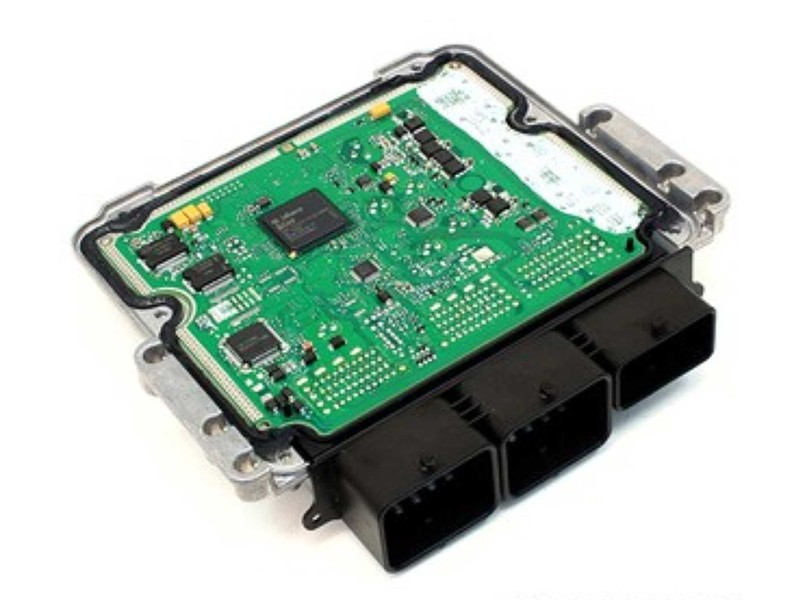
\includegraphics[height=1.5cm]{images/ecu.jpg}~~
		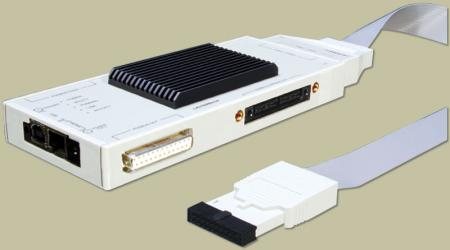
\includegraphics[height=1.5cm]{images/t32.jpg}~~
		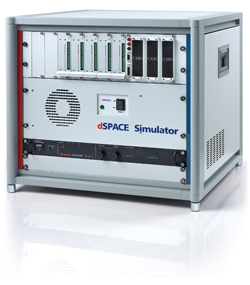
\includegraphics[height=1.5cm]{images/dspace.jpg}
		\caption{Technologies et outils utilisés}
	\end{figure}
	\vfill
	\pause
\vspace{-20px}
	\begin{block}{Gestion de projet}
		\begin{itemize}
			\item Réunions régulières
			\begin{itemize}
				\item Hebdomadaire avec mon tuteur
				\item Mensuelle avec le chef de groupe
				\item Dès que nécessaire avec l'équipe cliente
			\end{itemize}

			\item Développement court et itératif\newline
				\footnotesize $\Rightarrow$ Le client sera au centre du développement
		\end{itemize}
			\end{block}
\end{frame}
\subsection{Objectifs}
\begin{frame}{Objectifs du stage} 
	\begin{block}{Objectifs personnels}
	\begin{itemize}
		\item Prise de responsabilité sur le projet
		\item Découverte du multi-core
		\item Analyse des premiers retours d'utilisateurs
		\item Analyse des nouveaux besoins
	\end{itemize}
\end{block}
\pause
\begin{block}{Objectifs pour l'entreprise}
	\begin{itemize}
		\item Démocratiser l'utilisation de l'outil
		\item Améliorer les tests d'intégration du plugin
		\item Gagner du temps 
	\end{itemize}
\end{block}
\end{frame}


